\documentclass[12pt,oneside,a4paper]{article}

\usepackage[backend=biber,style=numeric]{biblatex}
\usepackage{xcolor}
\usepackage{todonotes}
\usepackage{amsmath}
\usepackage{braket}
\usepackage{multicol}
\usepackage{caption}
\usepackage{hyperref}
\usepackage{amssymb}
\usepackage{graphicx}
\usepackage{subcaption}
\usepackage{listings}
\usepackage[section]{placeins}
\lstdefinestyle{qasm}{
    belowcaptionskip=1\baselineskip,
    frame=top,frame=bottom,
    frameround=tttt,
    xleftmargin=\parindent,
    basicstyle=\footnotesize\ttfamily,
    tabsize=2,
    numbers=left,
    numbersep=5pt,
    stepnumber=1,
    columns=fullflexible,
}
\lstset{
	frame=top,frame=bottom,
	language=C,
	basicstyle=\small\normalfont,
	xleftmargin=\parindent,
	keywordstyle=\color{green!40!black},
    % FIXME remove this comments
	%  commentstyle=\itshape\color{purple!40!black},
	%  identifierstyle=\color{blue},
	%  stringstyle=\color{orange},
	morekeywords={in, globaldata, procedure, input, output, behavior, end, XOR, NOT, AND}, % keyword to highlight
	tabsize=2,
	numbers=left,
	stepnumber=1,                   % the step between two line-numbers.
	numbersep=5pt,
	framexleftmargin=10pt,
	title=\lstname,
	captionpos=t,
	showspaces=false,
}
\DeclareCaptionFormat{listing}{\rule{\dimexpr\textwidth\relax}{0.4pt}\par\vskip1pt#1#2#3}
\captionsetup[lstlisting]{format=listing,singlelinecheck=false, margin=0pt,labelsep=space,labelfont=bf}

\usepackage{booktabs}
\usepackage[noabbrev,capitalise]{cleveref}
\crefname{listing}{algorithm}{algorithms}
\Crefname{listing}{Algorithm}{Algorithms}
\renewcommand\lstlistingname{Algorithm}
\def\lstlistingcrefname{Algorithm}
\usepackage{url}

\addbibresource{assets/biblio.bib}

\title{\textbf{Quantum Circuit Simulation: A Unified Approach to Contraction, Compilation, and Execution on Heterogeneous Architectures}}

\author{Federico Lolli, Angelo Zangari}

\date{\today}

\begin{document}

\begin{titlepage}
    \centering
    \clearpage
    \maketitle
	\thispagestyle{empty}
	\vspace*{1cm}
	\vfill
	\centering
	
\includegraphics{logo_polimi.png}
\includegraphics{logo_NECST.png}
\end{titlepage}


\begin{abstract}
    In the rapidly evolving field of quantum computing, efficient simulation of quantum circuits on classical computers remains a critical challenge. This project focuses on developing a versatile and efficient simulation toolchain for quantum circuits, emphasizing compatibility with heterogeneous hardware architectures. Our approach centers on several key innovations that we believe can enhance the simulation process. At the core of our toolchain is a custom Instruction Set Architecture (ISA) that decomposes quantum circuits into a series of schedulable instructions, utilizing fundamental mathematical operators such as tensor expansions and matrix multiplications. This abstraction allows for flexible and efficient representation of quantum operations across various hardware platforms.
    We developed a prototype FPGA accelerator with custom kernels written specifically for these two operators, as a proof-of-concept to demonstrate the potential performance benefits of our approach. Our work aims to advance the field of quantum circuit simulation by providing a novel approach, concretized in a comprehensive, extensible toolchain that can adapt to various classical computing accelerators. While our current proof-of-concept targets FPGA implementation, the architecture of our toolchain lays the groundwork for efficient quantum circuit simulation on heterogeneous computing platforms, offering a powerful tool for researchers and developers in quantum computing.
\end{abstract}

\newpage
\tableofcontents

\newpage

%%%%%%%%%%%%%%%%%%%%%%%%%%%%%%%%%%%%%%%%%%%%%%%%%%%% SECTION 1

\section{Introduction}

\subsection{The Quantum Computing Landscape}

In recent years, the field of quantum computing has experienced significant advancements, promising to revolutionize computational capabilities for specific classes of problems. Quantum computers have the potential to solve certain tasks exponentially faster than their classical counterparts, particularly in areas such as cryptography \cite{Shor1995PolynomialTimeAF}, optimization \cite{Farhi2014AQA}, and quantum system simulations. However, the development and verification of quantum algorithms and circuits still heavily rely on classical computing resources.

\subsection{The Role of Classical Simulation}

Classical computers play a crucial role in the development of quantum computing technologies. They are extensively used for simulating and verifying quantum circuits, which is essential for:

\begin{itemize}
    \item Debugging and testing quantum algorithms
    \item Benchmarking quantum hardware performance
    \item Exploring the behavior of quantum systems at scales currently unattainable by physical quantum devices
\end{itemize}

Currently, popular frameworks like \textbf{Qiskit} \cite{qiskit2024} provide simulation capabilities with varying levels of performance. However, as quantum circuits grow in size and complexity, there is an increasing need for more efficient simulation techniques.

\subsection{Project Objectives}

The primary goal of this project is to develop a versatile and efficient simulation toolchain for quantum circuits, with a focus on compatibility with heterogeneous hardware while maintaining user-friendliness and integration with existing frameworks. Our key objectives can be summarized as follows:

\begin{enumerate}
    \item Design a comprehensive simulation toolchain for quantum circuits that can interface with various classical computing accelerators, including GPUs and FPGAs.
    \item Ensure interoperability with established quantum computing frameworks, particularly Qiskit, to integrate seamlessly into existing quantum development workflows.
    \item Develop a flexible representation of quantum operations that can be efficiently translated to different hardware architectures.
    \item Implement a prototype FPGA accelerator as a proof-of-concept to demonstrate the potential performance benefits of our approach.
    \item Establish a foundation for future research in heterogeneous quantum circuit simulation, allowing for easy extension to other accelerator architectures.
\end{enumerate}

Through these objectives, we aim to contribute to the advancement of quantum computing research by providing a powerful simulation toolchain that leverages the capabilities of heterogeneous computing architectures.

\subsection{Our Approach}

Our approach to quantum circuit simulation involves several key points:

\begin{itemize}
    \item \textbf{Whole circuit evaluation:} We aim to evaluate the whole circuit at once and the provide the resulting matrix, thus enabling the reuse of the matrix for successive experiments.
    \item \textbf{Use of well established standards:} By adhering to the QASM standard\cite{cross2017openquantumassemblylanguage} for quantum circuit representation we ensure compatibility with widely used quantum computing frameworks like Qiskit.
    \item \textbf{Instruction Set Architecture (ISA) Design:} We developed a custom ISA that decomposes quantum circuits into a series of instructions, enabling efficient representation and execution on various hardware platforms.
    \item \textbf{Tensor Network Contraction:} By employing tensor networks to represent quantum circuits and perform optimized contractions we aim to achieve efficient simulation in terms of computational complexity and memory usage \cite{pan2023efficientquantumcircuitsimulation}.
    \item \textbf{Sparse Matrix Operations:} We chose to represent quantum gate operands as sparse matrices (in COO format) and kept this format throughout the simulation to optimize memory usage and computational efficiency. We think that leveraging the sparsity of quantum states is crucial for efficient simulation of large circuits.
    \item \textbf{Compilation in an executable format:} We designed a compilation step that transforms the optimized contraction tree into a sequence of instructions compiled in a lightweight, portable binary format, representing the optimized computation plan. We also developed an interpreter to translate this binary format into the actual OpenCL operations to be executed on the FPGA.
    \item \textbf{Dynamic Scheduling:} Based on the optimized contraction path, we developed a scheduler that dynamically orders the instructions to maximize parallelism and minimize computational overhead.
    \item \textbf{FPGA Implementation:} We develop custom kernels from scratch, optimized for tensor expansion and matrix multiplication operations for COO sparse matrices on FPGAs to showcase the potential performance of accelerated quantum circuit simulation on heterogeneous architectures.
    \item \textbf{Use of memory safe compiled languages:} We implemented the entire simulation toolchain in Rust, leveraging its memory safety features and performance characteristics to ensure robustness and efficiency, along its extendability and maintainability.
\end{itemize}

\subsection{Report Structure}

The remainder of this report is organized as follows:

\begin{itemize}
    \item Section \ref{sec:background}: Provides necessary background information on quantum computing, tensor networks, and FPGA technology.
    \item Section \ref{sec:methodology}: Describes our simulation toolchain in detail, including the ISA design, tensor network contraction methods, and FPGA implementation.
    \item Section \ref{sec:results}: Presents the performance results of our implementation, comparing it with existing simulation methods.
\end{itemize}


%%%%%%%%%%%%%%%%%%%%%%%%%%%%%%%%%%%%%%%%%%%%%%%%%%%% SECTION 2

\section{Background}
\label{sec:background}

\subsection{What is quantum computing}
Quantum computing represents a revolutionary approach to information processing, fundamentally different from classical computing. It harnesses the principles of quantum mechanics to perform calculations, offering the potential to solve certain problems exponentially faster than traditional computers.
First of all, we introduce the concept of quantum states, which are complex vectors and in quantum mechanics notation are represented by "kets".
\begin{equation}
    \ket{\Psi} = \begin{bmatrix}
        \alpha\\
        \beta
    \end{bmatrix},
    \hspace{10 mm} \ket{\Psi} \in \mathbb{H}
\end{equation}
At the heart of quantum computing there are quantum bits, or qubits.
The qubit is the basic unit of quantum information; physically it's a two-state quantum-mechanical system, which simply means that it's an entity composed by two quantum states.
Unlike classical bits that can only be in one of two states (0 or 1), qubits can exist in a superposition of states, effectively encoding multiple classical states simultaneously. The superposition property allows quantum computers to process vast amounts of information in parallel. To achieve superposition the quantum states must form an orthonormal basis, or equivalently, they need to be able to span the entire two-dimensional Hilbert space of the qubit. For example, we can consider the orthonormal "kets" $\ket{0}$, $\ket{1}$; the superposition is mathematically described by a linear combination:
\begin{equation}
    \ket{\Psi} = \alpha \ket{0} + \beta \ket{1} = \alpha \begin{bmatrix} 1 \\ 0 \end{bmatrix} + \beta \begin{bmatrix} 0 \\ 1 \end{bmatrix},
    \hspace{10 mm} \alpha, \beta \in \mathbb{C}, \ket{\Psi}, \ket{1}, \ket{0} \in \mathbb{H}
\end{equation}

Note that $\alpha$, $\beta$ are the complex probability amplitudes of the qubit.


Quantum circuits, the building blocks of quantum computation, consist of quantum gates that manipulate qubits. These circuits differ significantly from classical circuits, which use high and low voltages to represent binary states. Instead, quantum circuits leverage quantum superposition to encode and process multiple states concurrently. In figure 1 \cite{quantumcircuit} we can see a quantum circuit with 5 qubits.
\begin{figure}[h]
    \centering
    \begin{subfigure}[b]{0.7\textwidth}
    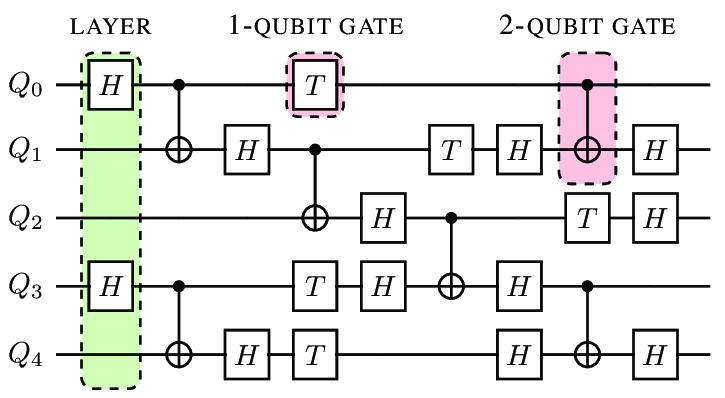
\includegraphics[width=\textwidth]{quantum_circuit.png}
    \end{subfigure}
    \caption{An example of quantum circuit}
\end{figure}

\subsection{What is a quantum gate}
Quantum gates are fundamental components in quantum computing, serving as the building blocks of quantum circuits. These gates are mathematical representations of unitary operations that manipulate quantum states, analogous to logic gates in classical circuits but with significantly different properties and capabilities.
Unlike classical gates that operate on definite binary states (0 or 1), quantum gates act on qubits, which can exist in superpositions of states. This key difference allows quantum gates to perform complex quantum operations that have no direct classical counterpart.
Gates are mathematically linear forms, and in quantum mechanic notation are represented by "bras".
\begin{equation}
    \bra{f} , \hspace{10 mm} f: V \rightarrow \mathbb{C}
\end{equation}
Gates can be applied to qubits using the braket notation, and the result is a complex number:
\begin{equation}
    \braket{f|v} \in \mathbb{C}
\end{equation}
The unitary nature of quantum gates ensures that the total probability of all possible outcomes remains conserved, a crucial property in maintaining the integrity of quantum information. These gates enable various transformations of quantum states, including rotations in the complex vector space, phase shifts, and entanglement operations between multiple qubits.
Quantum circuits are constructed by combining these quantum gates in specific sequences. While classical circuits use high and low voltages to represent and process binary information, quantum circuits leverage the quantum superposition principle to encode and manipulate multiple states simultaneously. This parallel processing capability is a key factor in the potential computational advantage of quantum systems.
The implementation of quantum gates allows for the execution of complex quantum algorithms. These algorithms can perform tasks such as quantum Fourier transforms, quantum error correction, and other operations that exploit the unique properties of quantum systems.
In essence, quantum gates are the operators that drive quantum computation, enabling the manipulation and transformation of quantum information in ways that are fundamentally different from classical information processing. Their ability to act on superpositions and create entanglement is central to the power and promise of quantum computing.

\subsection{Different approaches for quantum circuit simulation}
There are two main methods in quantum simulation: \\

The first one is state vector propagation, which is the traditional approach. It consists in computing the state vector of the circuit and propagating it through the circuit from the start to the end. This methodpresents severe limitations; mainly using a state vector to represent the circuit means that we need to store it, but the issue is that the vector dimension grows exponentially with respect to the number of circuit lanes. This renders the state vector method computationally infeasible from a spatial point of view for circuits with bigger dimension, roughly when the number of qubits exceeds 50.\\

The second method is newer and resorts to decomposing the quantum circuit into its corresponding tensor network representation. From here we can perform mathematical operations to contract the terms and get an equivalent expression of the circuit.
This method presents multiple great benefits:
\begin{itemize}
    \item It allows us to perform computations on subset of data, which can be contained on FPGAs.
    \item There are independent operations that can be scheduled in parallel.
    \item Decomposing the circuit in simpler operations allows for specific implementations (for instance specific kernels on FPGA).
\end{itemize}

\subsection{Tensor Network Methods}
A more recent approach involves decomposing the quantum circuit into its corresponding tensor network representation. In this method, quantum gates and initial states are represented as tensors and vectors, respectively. The circuit's structure is mapped to bonds between these tensors, creating a unique tensor network. Contracting this network yields a vector representing the final quantum state, containing amplitudes for the entire Hilbert space.\\

In particular, there are several approaches to take advantage of tensor networks for simulating quantum circuits. A brief explanation of them is necessary to understand the strenghts and weakness of each, and to understand where we place ourself in relation to them:
\begin{enumerate}
    \item Single Amplitude Simulation: Focuses on computing the amplitude of a single bitstring, with maximal restriction on the final state. Since all the tensors bonds are closed with the final bitstring, the result is directly its amplitude. Advantage of this method is the saving in memory complexity since by closing all tensors we avoid the need for the computation of the entire state vector of the circuit. The drawback is that the tensor constraction need to be repeated for each sampled bitstring.
    \item Full State Simulation: Aims to obtain all amplitudes in the entire Hilbert space, with no restrictions on the final state, by computing the entire state vector of the circuit. While this approach allows to compute the tensor contraction only once, it has the drawback of needing to store the entire state vector, which grows exponentially to the number of qubits of the circuit (for n qubits, the state vector has dimension $2^n$).
    \item Subspace Simulation: A middle ground approach, between single amplitude and full state simulation. It consists in choosing lanes which are not particularly relevant to the final bitstring computation and closing the bonds of the relative tensors, thus reducing the memory footprint while retaining the advantage of the single tensor contraction computation of the full state method.
\end{enumerate}

\newpage

\begin{figure}[h]
    \centering
    \begin{subfigure}[b]{0.3\textwidth}
    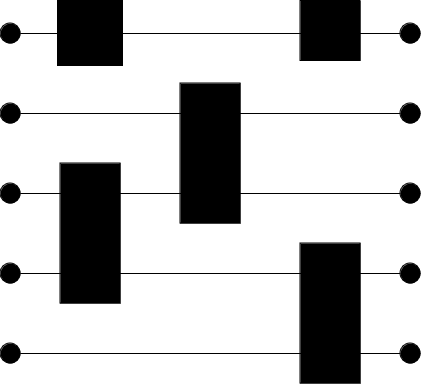
\includegraphics[width=\textwidth]{tn_single_amplitude.png}
    \caption{Single Amplitude\footnotemark[1]}
    \end{subfigure}
    \hfill
    \begin{subfigure}[b]{0.3\textwidth}
    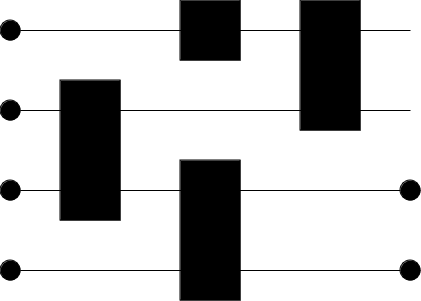
\includegraphics[width=\textwidth]{tn_subspace.png}
    \caption{Subspace\footnotemark[2]}
    \end{subfigure}
    \hfill
    \begin{subfigure}[b]{0.3\textwidth}
    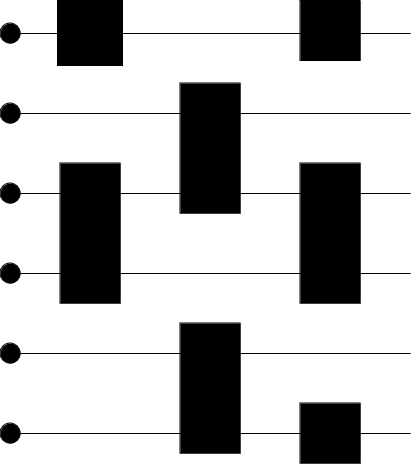
\includegraphics[width=\textwidth]{tn_full_state.png}
    \caption{Full State\footnotemark[3]}
    \end{subfigure}
    \caption{Tensor Network Simulation Approaches}
\end{figure}
\footnotetext[1]{Single amplitude simulation example}
\footnotetext[2]{Subspace simulation example}
\footnotetext[3]{Full state simulation example}

Our approach leans toward full state simulation; this was done because of multiple reasons. First of all, the single amplitude method requires the computation of the tensor contraction each time we need to simulate the circuit, which for large circuits becomes infeasible both computationally and economically. The subspace simulation method is was discarded due to the fact that we are devising a general method to simulate any quantum circuit, so we do not know a-prior what gates should be closed, because it depends on the specific quantum circuit. Because of that we went for the full state simulation approach, because of the following tradeoffs: even though there is the issue of storing the state vector in memory, we are dealing with highly sparse tensors, so although theorically the memory occupancy grows at $2^n$ w.r.t. the number of qubits, usually it will be much lower. Moreover, the modular structure and approach that we devised to tackle the problem (decomposing the circuit in tensors expansions and matrix multiplications) allows us to spread the memory load on multiple units both for storing and for computation (with techniques such as tiling).

\subsection{Tensor Expansion}
Is a mathematical operator through which two tensors originate a third one with rank the product of the rank of the input tensors. There are many algorithms to implement it, such as the Einsum notation, which compresses the indexes, or the kronecker product. We followed the latter, in which every element of the first matrix is multiplied by the entire second matrix and then be appropriately put in the result matrix.\\
To see the relative kernel implementation refer to section \ref{tens_exp_section}.

\subsection{Tensor Contraction}
Can be though as a generalization of a matrix multiplication. It can be performed between two tensors with same rank and spanning on exactly the same lanes, with no other quantum gates in between. The resulting tensor has the same dimensions (rank) as the starting tensors and each element can be computed as the traditional dot product between the appropriate row and column of the first and second matrix, respectively.
To see the relative kernel implementation refer to section \ref{matmul_section}.

\subsection{Sampling and evaluating quality of obtained sample with LXEB}
A note on circuit verification for completeness:\\
Our work poses as objective the computation of the tensor representing the final and contracted quantum circuit. This allows us to obtain a sample of the output bitstring simply by multiplying it for the input vector. After having computed the output tensor, and having obtained the bitstring amplitudes (what the researchers call Random Circuit Sampling (RCS) experiments), we can use verification to evaluate the quality of the results. To do this we simply compute the Linear Cross-Entropy Benchmark (LXEB) which compares the distribution of sampled bitstrings from the quantum device with the ideal theoretical distribution, providing a measure of how well the quantum computation aligns with expectations. To do this we simply sum the products of the probability of each bitstring in a noise-free circuit pU with the probability in a real one q(x).

\begin{equation}
    F_l = 2^N \sum_x p_U(x)q(x) - 1 = 2^N E_{x \sim q(x)} p_U(x) - 1
\end{equation}

Since obtaining all the bistring for computing q(x) is infeasible, we compute the LXEB for a randomically sampled subset of bitstring, with cardinality $m$.

\begin{equation}
    F_l = 2^N \sum_{i=1}^m p_U(x_i)/m - 1.
\end{equation}

The obtained $F_l$ is the LXEB score of the circuit, which is usually expressed in percentage.

\subsection{Challenges}
While tensor network methods offer significant advantages for quantum circuit simulation, they also present several challenges that need to be addressed for effective implementation, the main ones being:
\begin{itemize}
    \item Contraction Path Finding: The identification of an optimal contraction path for tensor networks is NP-hard. With numerous tensors involving multiple dimensions, finding the most efficient contraction sequence becomes increasingly difficult as the circuit size grows. Recent advancements in path-finding approaches revolve around graph-partitioning and simulated annealing (SA).
    \item Sparsity: Quantum states in larger circuits often exhibit high sparsity, meaning that many amplitudes are zero or near-zero. Efficiently handling this sparsity in tensor network contractions is crucial for performance optimization and memory management.
    \item Precision Requirements: Quantum simulations often require high numerical precision to maintain accuracy, especially in cases where small amplitude differences are significant. This requirement can lead to computational challenges, for instance when dealing with numerical cancellation in complex calculations.
    \item Scalability: As quantum circuits grow in size and complexity, the computational resources required for simulation increase dramatically. Balancing the trade-off between simulation accuracy and computational feasibility becomes increasingly challenging.
    \item Memory Management: Tensor network methods can be memory intensive, especially for larger circuits. Efficient memory allocation and management are critical to prevent bottlenecks and enable simulation of more complex quantum systems.
    \item Parallelization and Hardware Optimization: Leveraging parallel computing architectures and optimizing for specific hardware (like FPGAs or GPUs) requires careful algorithm design and implementation to fully exploit the potential performance gains.
\end{itemize}

Addressing these challenges is crucial for advancing the field of quantum circuit simulation. Ongoing research focuses on developing more efficient contraction algorithms, improving numerical stability, and optimizing implementation for various hardware architectures. These efforts aim to bridge the gap between the theoretical capabilities of tensor network methods and their practical implementation in simulating increasingly complex quantum circuits.


%%%%%%%%%%%%%%%%%%%%%%%%%%%%%%%%%%%%%%%%%%%%%%%%%%%% SECTION 3

\section{Methodology}
\label{sec:methodology}

Our toolchain consists of two key components:

\begin{itemize}
    \item \textbf{Frontend:} Responsible for parsing quantum circuits, converting them into tensor networks, generating contraction plans, and compiling them into an optimized sequence of instructions. It's the high-level interface between the user and the simulation process.
    \item \textbf{Backend:} Executes the compiled instructions on the target hardware, performing tensor expansions and matrix multiplications to compute the whole circuit unitary matrix. It's the low-level computational engine that drives the simulation process.
\end{itemize}

The frontend is built with expandability and compatibility in mind, allowing for easy integration with existing quantum computing frameworks and interaction with various computational backends. The backend is designed to efficiently execute the compiled instructions on different hardware platforms, leveraging the unique capabilities of each architecture. Together, these components form a comprehensive simulation toolchain that can adapt to diverse quantum computing research needs.

\subsection{Frontend}
% TODO highlight the implementation of x86 ISA

The Frontend is a fundamental component in the quantum circuit simulation process, serving as the interface between high-level quantum circuit descriptions and low-level computational backends. By reducing the quantum circuit to a tensor network and optimizing the contraction tree, the frontend prepares the circuit for efficient simulation with minimum number of operations. Without this crucial step, the computational backends would be unable to efficiently simulate quantum circuits, leading to significant performance degradation and resource wastage.

All the code employed in the frontend is hosted on GitHub at the following \href{https://github.com/federico123579/HPPS24-Quantum-Simulation}{repository}, feel free to contact the authors if you haven't access to it.

This section presents the architecture, functionality, and implementation details of the frontend, presenting at the end a compilation example to illustrate the process.

\subsubsection{Architectural Overview and Core Functionality}

The principal objective of the frontend is to transform a high-level quantum circuit description into an optimized sequence of instructions for efficient simulation. This process involves several key stages, each explained more in detail forward:

\begin{enumerate}
    \item \textbf{Parsing} of a high-level quantum circuit description language (QASM) into an internal representation
    \item \textbf{Conversion} of the quantum circuit into a \textbf{Tensor Network}, highlighting available tensor contractions
    \item \textbf{Generation} of an optimized contraction tree, packed in a \textbf{Contraction Plan} (\textbf{CP}) structure (for CPU backends, where each contraction can be executed as a single Einsum operation), or an \textbf{Operation Tree} (\textbf{OT}) realized in an \textbf{Operation Plan} (\textbf{OP}) structure (for FPGA backends, where the contraction is split into multiple operations).
    \item \textbf{Compilation} of the generated plan (CP/OP) in a set of instructions with explicit dependencies, based on a backend-specific \textbf{Instruction Set Architecture} (\textbf{ISA}).
    \item \textbf{(QCF) Compilation} of the optimized instructions into a lightweight, portable binary format (\textbf{Q}uantum \textbf{C}omputation \textbf{F}ormat), ready for execution on the chosen backend.
    \item \textbf{Scheduling} of instructions for optimal execution, exploiting independency between leaves of the contraction tree and maximizing instruction-level parallelism.
\end{enumerate}

\subsubsection{Circuit Parsing and Representation}

The initial phase of the frontend's operation involves parsing a QASM 3.0\cite{cross2017openquantumassemblylanguage} file. Our parser implementation supports a subset of the QASM 3.0 specification, focusing on the essential elements required to parse QisKit\cite{qiskit2024} randomly generated circuits. Specifically, it supports all standard gates included in the \href{https://github.com/Qiskit/qiskit/blob/main/qiskit/qasm/libs/stdgates.inc}{\texttt{stdgates.inc}} library, custom gate definitions within the QASM file, while excluding certain advanced features such as measurement operations and classical control structures.

Following the parsing phase, the frontend constructs an internal representation of the quantum circuit. This internal model serves as the foundation for subsequent compilation stages.

\subsubsection{Tensor Network Conversion}

The next crucial stage involves the transformation of the quantum circuit into a tensor network. This process comply with the following rules:

\begin{itemize}
    \item Each quantum gate is mapped to a corresponding tensor, preserving its quantum operational semantics.
    \item Connections between gates are represented as tensor contractions, reflecting the flow of quantum information through the circuit.
\end{itemize}

The resulting structure is a graph where edges represent tensors and nodes represent tensor contractions.

The rules for drawing contraction arcs in the tensor network follow established conventions in quantum tensor network theory \cite{biamonte2017tensornetworksnutshell}. These rules ensure that the tensor network accurately represents the quantum circuit's operations and qubit interactions.

\subsubsection{Contraction Tree Generation}

From the tensor network representation, the frontend generates a contraction tree using a custom algorithm. This binary tree structure represents the optimal order of tensor contractions:

\begin{itemize}
    \item Leaf nodes represent individual tensors, corresponding to quantum gates in the original circuit.
    \item Internal nodes represent contraction operations between tensors.
    \item The tree structure is optimized to minimize the total number of operations required to compute the final quantum state.
\end{itemize}

Our custom algorithm for generating the contraction tree is based on a heuristic approach that balances computational efficiency with contraction order optimization. While the detailed description of this algorithm is beyond the scope of this section, it can be summarized as a recursive process that identifies the most efficient contraction order based on tensor dimensions and connectivity.

Once the contraction tree is constructed, it is encapsulated in a Contraction Plan (CP) structure, which serves as the blueprint for subsequent compilation stages.

In case the backend is an FPGA, the contraction tree is transformed into an Operation Tree (OT) structure, subdividing the contractions into equivalent multiple operations that can be executed on the FPGA. This transformation is necessary to adapt the contraction tree to the specific capabilities and constraints of the FPGA backend. This further step led to a Operation Plan (OP), sharing the same interface as the CP.

\subsubsection{Compilation and Instruction Scheduling}

The generated plan is subsequently converted to a set of instructions based on a backend-specific Instruction Set Architecture (ISA) (see subsection~\ref{subsec:isa}). Then is compiled in a lightweight, portable binary format (QCF), ready for execution on the chosen backend.

A scheduler is employed to optimize the order of instructions in the set derived from the contraction plan, maximizing instruction-level parallelism and minimizing computational overhead. This scheduling process controls the execution flow of the quantum circuit simulation, in a dynamic and adaptive manner by employing a dependency graph constructed from the contraction plan. The scheduler uses and updates this graph to determine the optimal instruction sequence.

\subsubsection{Backend Interface}

The frontend is architected to support multiple computational backends, while currently supporting a CPU executor and a prototypal FPGA accelerator. The final ISA instructions are transmitted to the chosen backend for execution, controlled by the scheduler and optimized for the specific hardware architecture.

The communication between the Rust-based frontend and the FPGA backend is planned to be implemented using OpenCL Rust bindings. This communication layer is currently under development, while the link between the host and the FPGA is based on a custom binary file format read once and executed in order (without dynamic scheduling).

\subsubsection{Implementation Details}

The entire frontend is implemented in Rust, taking advantage of the robust type system and memory safety features the language offers. This choice offers several significant advantages:

\begin{itemize}
    \item Enhanced reliability through compile-time error checking, reducing the likelihood of runtime errors.
    \item Improved maintainability and extensibility of the codebase, facilitated by Rust's modern language features and clear ownership model.
    \item Efficient parallelization for the CPU backend using the \href{https://github.com/rayon-rs/rayon}{\texttt{rayon}} parallel computing library.
\end{itemize}

Rust's strong typing and borrow checker have been particularly beneficial in implementing the tensor network operations, ensuring memory safety in complex data transformations without sacrificing performance and boosting productivity, thanks to many errors avoided at compile time.

\subsubsection{Compilation Example}

Let us take the Quantum Fourier Transform (QFT)\cite{coppersmith2002approximatefouriertransformuseful} circuit as an example. The QFT circuit is a fundamental quantum algorithm that transforms a quantum state into its Fourier representation. The QFT circuit is represented in QASM as follows:

\begin{lstlisting}[style=qasm, caption={QFT Circuit in QASM}]
	qubit[4] q;
	x q[0];
	x q[2];
	barrier q;
	h q[0];
	cphase(pi / 2) q[1], q[0];
	h q[1];
	cphase(pi / 4) q[2], q[0];
	cphase(pi / 2) q[2], q[1];
	h q[2];
	cphase(pi / 8) q[3], q[0];
	cphase(pi / 4) q[3], q[1];
	cphase(pi / 2) q[3], q[2];
	h q[3];
\end{lstlisting}

% add figure of the tensor network

In figure~\ref{fig:tensor-network}, we present the tensor network representation of the QFT circuit. In this illustration of the tensor network, each node represents a tensor, along what we define as \textbf{span} (the qubits it acts on), and each edge represents a qubit connection between tensors, where an eventual contraction will take place.

Possible contractions can be identified by edges characterized by the same \textbf{span} as the intersection of the \textbf{spans} of the two tensors they connect (highlighted in red and green in the figure).

Each contraction has a cost associated with it, defined by the \textbf{rank} of the operation tied to the contraction. With the word \textbf{rank} we refer to the number of qubits involved in the operation. The cost of a contraction depends on the number of qubits involved in the operation, with higher ranks incurring higher costs (in terms of computational complexity). In the figure two colors, one lighter than the other, have been used to identify nodes (gates) of rank one and greater, respectively.

\begin{figure}
    \centering
    \begin{minipage}{.45\textwidth}
        \centering
        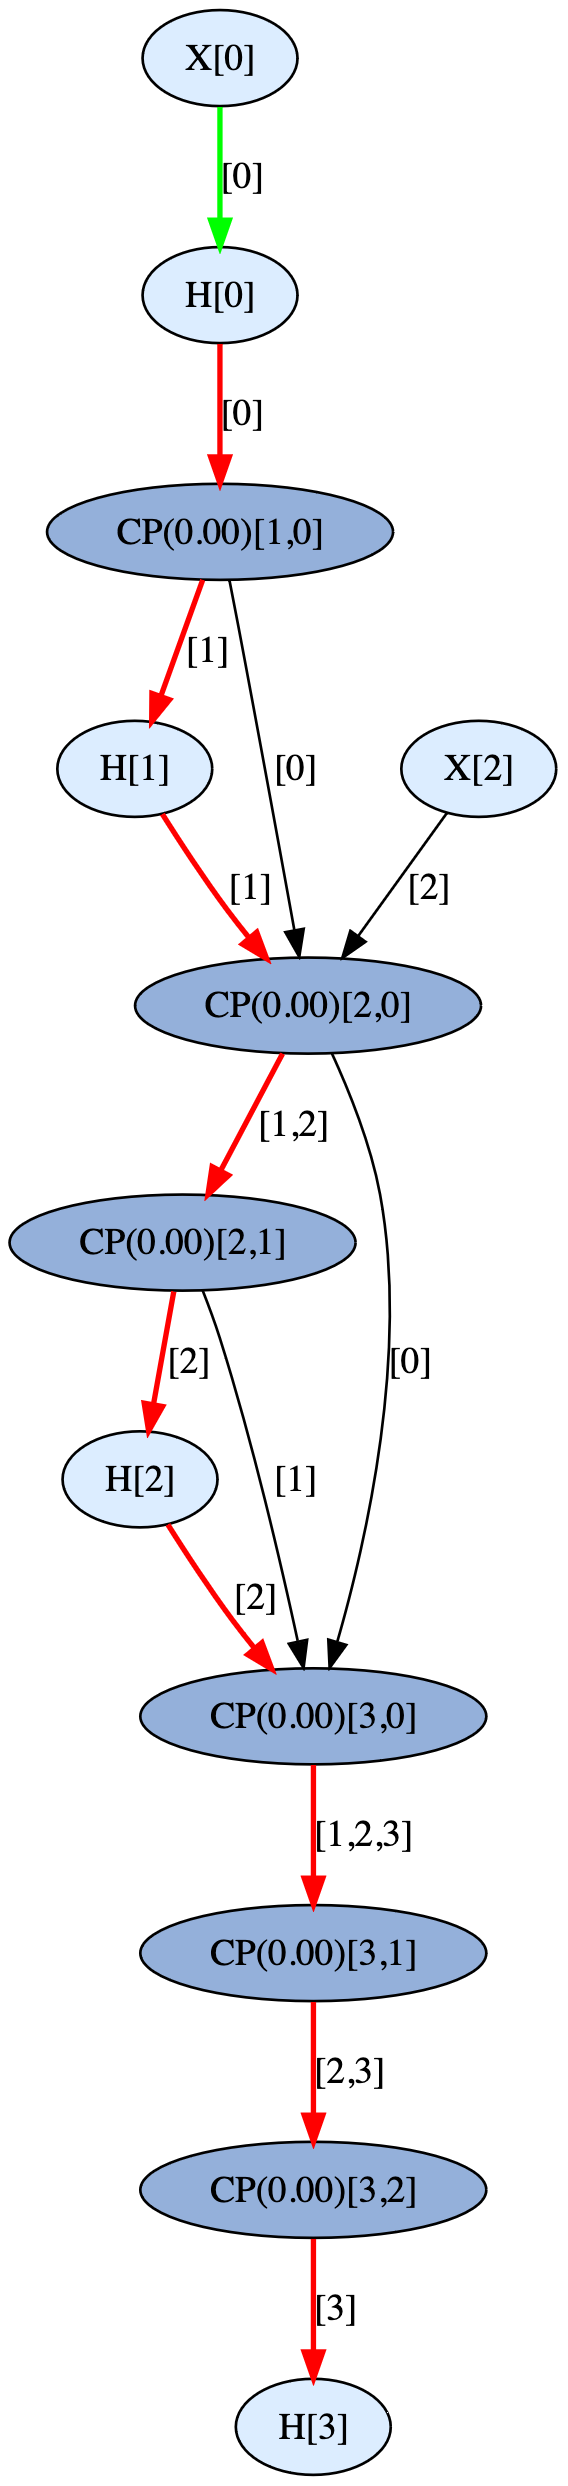
\includegraphics[width=.6\textwidth]{tensor_network.png}
        \caption{Tensor Network Representation of the QFT Circuit}
        \label{fig:tensor-network}
    \end{minipage}%
    \hfill
    \begin{minipage}{.45\textwidth}
        \centering
        \begin{tabular}{c}
            $\texttt{000: M(02x02)}\;\odot\;\texttt{M(02x02)}$ \\
            $\texttt{001: I(00000)}\;\otimes\;\texttt{M(02x02)}$ \\
            $\texttt{002: I(00001)}\;\odot\;\texttt{M(04x04)}$ \\
            $\texttt{003: M(02x02)}\;\otimes\;\texttt{M(02x02)}$ \\
            $\texttt{004: I(00002)}\;\odot\;\texttt{I(00003)}$ \\
            $\texttt{005: I(00004)}\;\otimes\;\texttt{M(02x02)}$ \\
            $\texttt{006: M(04x04)}\;\otimes\;\texttt{M(02x02)}$ \\
            $\texttt{007: I(00006)}\;\odot\;\texttt{M(08x08)}$ \\
            $\texttt{008: I(00005)}\;\odot\;\texttt{I(00007)}$ \\
            $\texttt{009: M(02x02)}\;\otimes\;\texttt{M(02x02)}$ \\
            $\texttt{010: M(04x04)}\;\odot\;\texttt{I(00009)}$ \\
            $\texttt{011: M(02x02)}\;\otimes\;\texttt{I(00010)}$ \\
            $\texttt{012: I(00008)}\;\odot\;\texttt{I(00011)}$ \\
            $\texttt{013: I(00012)}\;\otimes\;\texttt{M(02x02)}$ \\
            $\texttt{014: M(02x02)}\;\otimes\;\texttt{M(08x08)}$ \\
            $\texttt{015: M(16x16)}\;\odot\;\texttt{I(00014)}$ \\
            $\texttt{016: M(02x02)}\;\otimes\;\texttt{M(02x02)}$ \\
            $\texttt{017: M(04x04)}\;\odot\;\texttt{I(00016)}$ \\
            $\texttt{018: M(04x04)}\;\otimes\;\texttt{I(00017)}$ \\
            $\texttt{019: I(00015)}\;\odot\;\texttt{I(00018)}$ \\
            $\texttt{020: I(00013)}\;\odot\;\texttt{I(00019)}$
        \end{tabular}
        \caption{Operation Plan for the QFT Circuit}
        \label{fig:operation-plan}
    \end{minipage}
\end{figure}

\begin{figure}
    \centering
    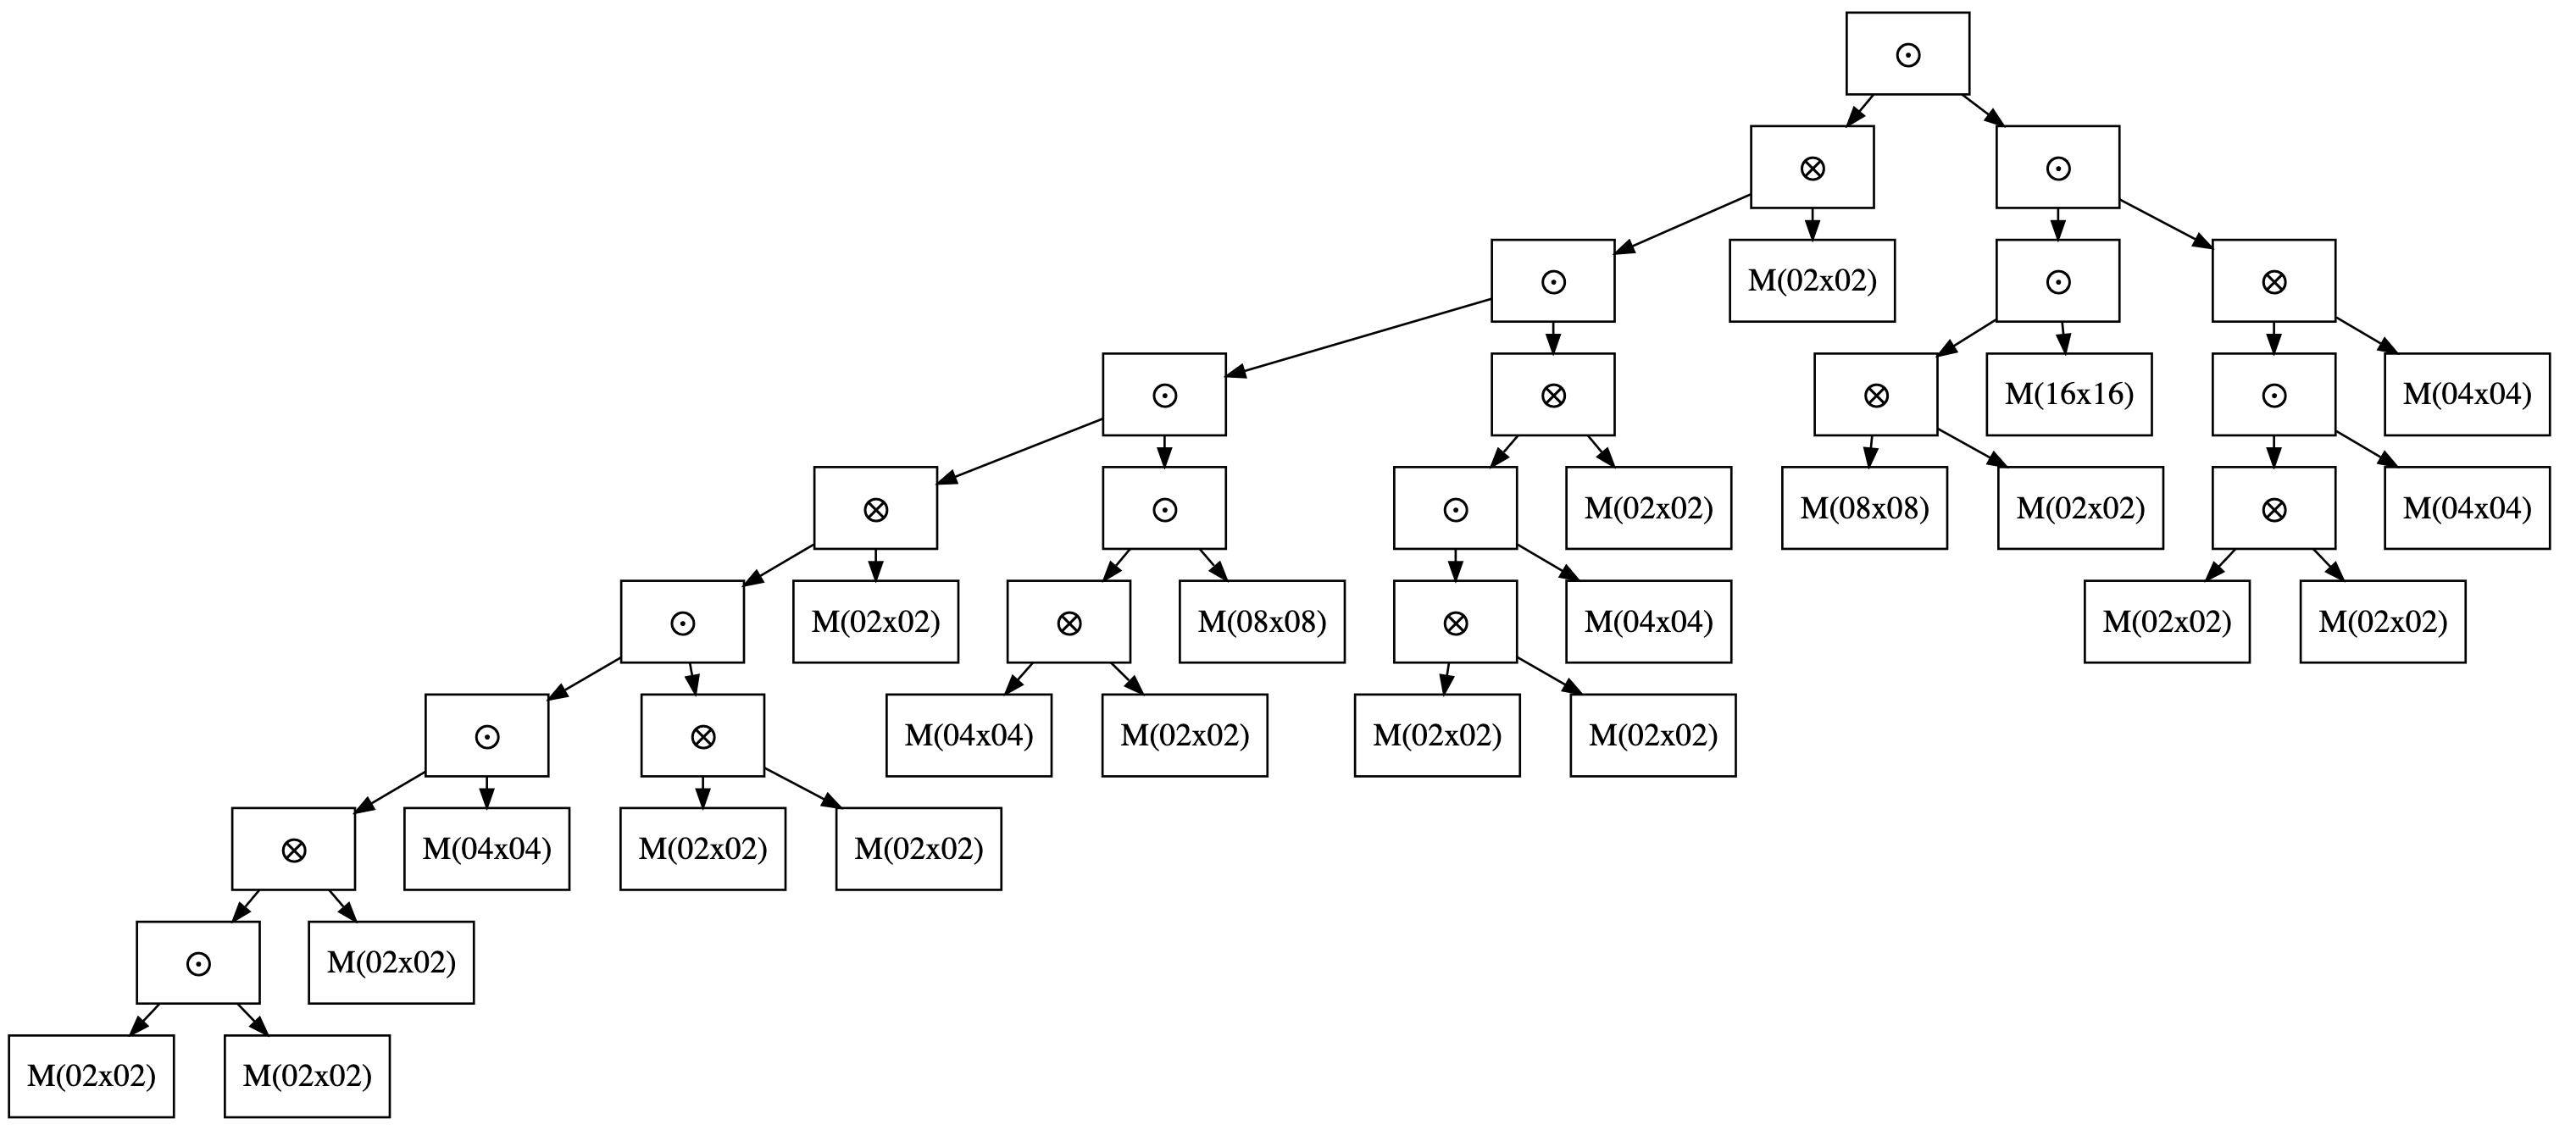
\includegraphics[width=\textwidth]{operation_tree.png}
    \caption{Operation Tree for the QFT Circuit}
    \label{fig:operation-tree}
\end{figure}

Highlighted in green is the contraction that will be performed first, as it has the lowest cost (rank 1, involving only 1 qubit). The contractions highlighted in red will be re-evaluated in another \textbf{sweep} of the algorithm, that is the process of identifying the optimal contraction path.

Starting from the tensor network, the frontend will go through a series of intermediate steps, eventually leading to the generation of an \textbf{Operation Tree} (OT) (figure~\ref{fig:operation-tree}) and its subsequent \textbf{Operation Plan} (Op) (figure~\ref{fig:operation-plan}). This plan is fed to the scheduler, that will optimize the order of the operations to send to the backend for execution.

Each instruction can be seen as a tensor operation, with the format:

\begin{center}
    \texttt{<ID>: <T1> <OP> <T2>}
\end{center}

Where \texttt{<ID>} is the instruction identifier, \texttt{<T1>} and \texttt{<T2>} are the tensors involved in the operation, and \texttt{<OP>} is the operation to be performed (e.g., $\otimes$ for tensor expansion and $\odot$ for matrix multiplication). The tensor operands can be identified either directly by matrix dimensions or by the address, if the the operation has a dependency on a previous instruction.

\FloatBarrier

\subsubsection{Future Work and Optimizations}

While the current implementation provides a robust foundation, several areas for future improvement have been identified:

\begin{itemize}
    \item Extending QASM support to full specification compliance
    \item Optimizing the contraction tree generation algorithm employing advanced graph based techniques \cite{PhysRevE}
    \item Implementing and optimizing the OpenCL communication layer for FPGA and GPU backends
    \item Exploring advanced scheduling techniques for improved instruction-level parallelism
\end{itemize}

Potential optimization strategies include the implementation of a hybrid CPU-FPGA approach for dynamic workload distribution and the exploration of quantum-inspired classical algorithms for improved tensor network contraction.

By continually refining and expanding the frontend's capabilities, we aim to create a versatile and efficient quantum circuit simulation framework that can leverage various backend architectures and implementations.

\subsection{Instruction Set Architecture (ISA) Design}
\label{subsec:isa}

An Operation Plan (OP) can be compiled into a set of instructions described better in the following table:

\begin{table}[t]
	\caption{ISA for computations on the FPGA backend}
	\centering
	\resizebox{.7\textwidth}{!}{\begin{tabular}{cccc}
		\toprule
		\textbf{Instruction} & \textbf{Opcode} & \textbf{Left Operand} & \textbf{Right Operand}\\
		\midrule
		\texttt{TE(MxM)} & \texttt{0x01} & \texttt{CooMatrixFmt} & \texttt{CooMatrixFmt} \\
        \texttt{TE(MxA)} & \texttt{0x02} & \texttt{CooMatrixFmt} & \texttt{AddressFmt} \\
        \texttt{TE(AxM)} & \texttt{0x03} & \texttt{AddressFmt} & \texttt{CooMatrixFmt} \\
        \texttt{TE(AxA)} & \texttt{0x04} & \texttt{AddressFmt} & \texttt{AddressFmt} \\
        \texttt{MM(MxM)} & \texttt{0x05} & \texttt{CooMatrixFmt} & \texttt{CooMatrixFmt} \\
        \texttt{MM(MxA)} & \texttt{0x06} & \texttt{CooMatrixFmt} & \texttt{AddressFmt} \\
        \texttt{MM(AxM)} & \texttt{0x07} & \texttt{AddressFmt} & \texttt{CooMatrixFmt} \\
        \texttt{MM(AxA)} & \texttt{0x08} & \texttt{AddressFmt} & \texttt{AddressFmt} \\
		\bottomrule
	\end{tabular}}
	\label{tab:isa}
\end{table}

The Instruction Set Architecture (ISA) described in table~\ref{tab:isa} is designed to support the execution of tensor expansion (\texttt{TE}) and matrix multiplication (\texttt{MM}) operations on the FPGA backend. The ISA defines a set of opcodes that correspond to specific tensor operations, each with distinct operand formats. The operands are represented in custom formats:

\begin{itemize}
    \item \texttt{CooMatrixFmt}: Represents a matrix in Coordinate (COO) sparse format, containing non-zero values and their corresponding row and column indices. To see the full definition of the format, refer to the table~\ref{tab:coo-matrix-fmt}.
    \item \texttt{AddressFmt}: Represents the memory address of a matrix in the FPGA memory space, by encoding a single 32-bit address in little-endian format.
\end{itemize}

\begin{table}
    \caption{COO Matrix Format}
    \centering
    \resizebox{.9\textwidth}{!}{\begin{tabular}{lcc}
        \toprule
        \textbf{Value} & \textbf{Format} & \textbf{Amount} \\
        \midrule
        number of non zero elements (\texttt{NZ}) & \texttt{uint32\_t} & \texttt{1} \\
        rank of the tensor & \texttt{uint8\_t} & \texttt{1} \\
        format (col-major or row-major) & \texttt{uint8\_t} & \texttt{1} \\
        element value & \texttt{CooElementFmt~\ref{tab:coo-el-fmt}} & \texttt{NZ} \\
        \bottomrule
    \end{tabular}}
    \label{tab:coo-matrix-fmt}
\end{table}


\begin{table}
    \caption{COO Element Format}
    \centering
    \resizebox{.5\textwidth}{!}{\begin{tabular}{lcc}
        \toprule
        \textbf{Value} & \textbf{Format} & \textbf{Amount} \\
        \midrule
        row index & \texttt{uint32\_t} & \texttt{1} \\
        column index & \texttt{uint32\_t} & \texttt{1} \\
        real & \texttt{float} & \texttt{1} \\
        imaginary & \texttt{float} & \texttt{1} \\
        \bottomrule
    \end{tabular}}
    \label{tab:coo-el-fmt}
\end{table}

\FloatBarrier

\subsection{Backend}

This section provides an in-depth overview of the FPGA backend, focusing on the architectural design and optimization strategies employed in kernel design. Since the development of both the FPGA kernels has been done from scratch, after months of research and development devoted to the development and optimization of the frontend, the backend currently lacks the same level of maturity and polish. However, being the FPGA backend a crucial component of the toolchain, we focused on delivering a functional prototype that can be further refined and optimized in future iterations.

All the code employed in the backend is hosted on GitHub at the following \href{https://github.com/angelozangari/HPPS24-Tensor-Contraction-HLS}{repository}, feel free to contact the authors if you haven't access to it.

\subsubsection{Architectural Overview}

Our FPGA-based acceleration solution comprises two primary kernels, each tailored for a specific mathematical operation described in the ISA previously presented:

\begin{enumerate}
    \item \textbf{Tensor Expansion Kernel}: Implements the Kronecker product operation between two sparse (COO) matrices of variable dimensions, used in tensor expansion operations.
    \item \textbf{Matrix Multiplication Kernel}: Performs sparse (COO) matrix multiplication for tensor contractions.
\end{enumerate}

Both kernels are designed to operate on matrices represented in the Coordinate (COO) sparse format, meeting strict memory constraints and ensuring efficient memory access patterns. Choosing the right sparse format is fundamental for a feasible FPGA implementation\cite{FormatsHwSpMsurvey}, as it allows for reduced memory bandwidth requirements and improved computational density, at the cost of dynamic and imperfect loop structures. Choosing COO format allows the kernels to be used transparently with both row-major and column-major matrices, by simply changing the order of the elements in the input stream. The advantages of this approach will be further discussed in the following sections.

\subsubsection{Implementation Details}

The kernels have been implemented \textit{ex novo} using Vitis High-Level Synthesis (HLS), without relying on external libraries beyond the standard Vitis HLS includes. This approach brought several challenges, the strict hardware constraints made the design process more complex, and different trade-offs had to be considered, but it also allowed for a more tailored and optimized implementation.

\subsubsection{Tensor Expansion Kernel} \label{tens_exp_section}

\begin{figure}[h]
    \centering
    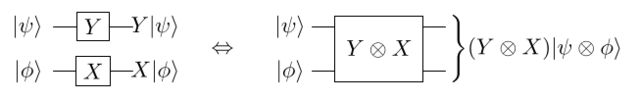
\includegraphics[width=.9\textwidth]{parallel_gates.png}
    \caption{Tensor Expansion operation on Quantum Qubits}
    \label{fig:tensor-expansion}
\end{figure}

The Tensor Expansion kernel implements the Kronecker product of two arbitrarily large matrices (obviously bounded by DRAM constraints). This operation is applied on parallel gates (that is gates that act on different qubits) in the quantum circuit, and it is required to elevate the rank of a gate (increasing its dimensions) to match the rank of the gate it has to be contracted with, while preserving the quantum semantics of the circuit.

\subsubsection{Matrix Multiplication Kernel} \label{matmul_section}

\begin{figure}[h]
    \centering
    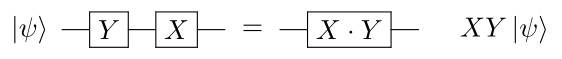
\includegraphics[width=.7\textwidth]{serial_gates.png}
    \caption{Matrix Multiplication operation on Quantum Qubits}
    \label{fig:matrix-multiplication}
\end{figure}

The Matrix Multiplication kernel performs the multiplication of two sparse matrices in COO format, this operation has to be interpreted as the equivalent gate from two gate in series. To efficiently operate on a stream of COO elements, the kernel is designed to accept left input elements by rows and right input elements by columns. This design choice ensures that the kernel can handle both row-major and column-major matrices transparently (by swapping the input order).

A notable aspects of the Matrix Multiplication kernel is the implementation of a packet-based approach to efficiently handle sparse matrix multiplication. The kernel allows to change the packet size according to needs (with the preprocessor directive \texttt{PACKET\_SIZE}).

% FIXME what do you mean by: " Optimization for the inherently imperfect loop structures resulting from the sparse COO format. " ?

\subsubsection{Optimization Strategies}

Several optimization techniques have been employed to maximize the performance of our FPGA kernels:

\begin{enumerate}
    \item \textbf{Dataflow Optimization}: Both the kernels have been defined as dataflow kernels, as suggested by the HLS best practices. This allows for a more efficient use of the FPGA resources and a better exploitation of the parallelism available in the problem.
    \item \textbf{Producer-Consumer Pattern}: HLS streams have been used extensively in the kernels, producer-consumer pattern is at the core of the implementation, enabling correct pipelining of the inner loop, our primary concern.
    \item \textbf{Packet-Based Processing}: Employed in the Matrix Multiplication kernel to operate on fixed-size packets of non-zero elements, paving the way to efficient sparse matrix multiplication of arbitrary dimensions without incurring significant memory overhead.
    \item \textbf{Memory constraint awareness}: Exclusive use of sparse matrix formats is a key requirement in this field, since few qubits more can be exponentially penalizing in terms of memory requirements.
\end{enumerate}

\subsubsection{Integration and Data Flow}

The integration of the FPGA kernels with the host side is facilitated through OpenCL, enabling seamless data transfer and kernel invocation. At the moment the communication with OpenCL can be performed by leveraging a different executable that reads the QCF file and sends the instructions to the FPGA, but the plan is to integrate the communication layer directly into the frontend, to allow for dynamic scheduling and workload distribution.

\subsubsection{Future Work and Optimizations}

While the current implementation provides a valid starting point, several areas for future improvement have been identified:

\begin{enumerate}
    \item Implementation of multiple Processing Elements (PEs) for the sparse matrix multiplication kernel to further increase parallelism.
    \item Exploration of dynamic indexing schemes for the Tensor Expansion kernel to improve flexibility and efficiency for varying input sizes.
    \item Investigation of fixed-precision arithmetic to optimize the trade-off between accuracy and performance.
    \item Development of a more sophisticated OpenCL-based communication layer to enable dynamic scheduling and workload distribution between the host and FPGA.
\end{enumerate}

By continuing to refine and optimize our FPGA kernel implementations, we aim to deliver a high-performance and scalable solution that can compete with current state-of-the-art quantum circuit simulation GPU implementations, highlighting the unique advantages of FPGA acceleration in this domain.

%%%%%%%%%%%%%%%%%%%%%%%%%%%%%%%%%%%%%%%%%%%%%%%%%%%% SECTION 4

\section{Results}
\label{sec:results}

\subsection{Setup}
% what was run and on which architecture (to allow others to replicate results)
% - tests in local:
% 	- clone repo
% 	- install cmake, just and other requirements
% 	- ... run tests, look at justfile or type just into terminal
% - vitis hls
% 	- which version
% 	- ...
% - vivado/opencl
% 	- version
% 	- parameters to compile kernel (clock frequency, board - alveo u55c, ...)
% 	- ...
% - Describe the experimental setup:
% - Hardware specifications (CPU, FPGA model)
% - Software versions (Vitis HLS, Vivado/OpenCL)
% - Compilation parameters (clock frequency, target board - Alveo U55C)
% - Instructions for reproducing the setup (cloning repo, installing dependencies)

\subsection{Results and comparisons}

\section{Results}

\subsection{Analysis of Tensor Network Contractions Effectiveness}

Our analysis focused on three key measurements: contraction time, execution time, and time gained through optimization techniques. To better showcase how the tensor network contractions approach outperform the normal execution. We examined these metrics across different circuit depths and qubit counts (5, 6, and 7 qubits).

This benchmark has been conducted on a local machine with an Intel Core i5-14600k CPU (single-thread), testing randomly generated circuits with varying depths and qubit counts (using the Qiskit library). Depth has been varied from 50 to 500 (incrementing by 10 each time), while qubit count has been set to 5, 6, and 7.

\subsubsection{Contraction Time vs Circuit Depth}

\begin{figure}[h]
    \centering
    \includegraphics[width=0.8\textwidth]{depth_vs_contraction_time.png}
    \caption{Contraction time vs circuit depth}
    \label{fig:contraction_time}
\end{figure}

For all qubit counts (5, 6, and 7), contraction time increases linearly with circuit depth and the rate of increase is higher for larger qubit counts, reasonably due to the higher number of tensor contractions required and dimensionality explosion. Still a linear relationship is maintained, allowing for predictable scaling of computational resources.

\subsubsection{Execution Time vs Circuit Depth}

\begin{figure}[h]
    \centering
    \includegraphics[width=0.8\textwidth]{depth_vs_execution_time.png}
    \caption{Execution time vs circuit depth}
    \label{fig:execution_time}
\end{figure}

Execution time also increases linearly with circuit depth, but at a higher rate compared to contraction time. This is expected, as the execution time includes additional operations beyond tensor contractions, such as matrix multiplications and tensor expansions. The gap between contraction time and execution time widens as circuit depth increases, highlighting how the contraction-based optimization technique outperforms the normal execution method.

\subsubsection{Time Gained vs Circuit Depth}

\begin{figure}[h]
    \centering
    \includegraphics[width=0.8\textwidth]{depth_vs_time_gained.png}
    \caption{Time gained vs circuit depth}
    \label{fig:time_gained}
\end{figure}

The time gained through the contraction method compared to the normal method is most pronounced for 7-qubit circuits, with substantial increases observed as circuit depth increases. While the overhead cost for lower qubit counts (5 and 6) is minimal, but present, the benefits of the contraction method become more evident for larger quantum systems. The time gained rises rapidly up to a circuit depth of about 350, after which it plateaus at around 6 seconds. This plateau suggests an upper limit to the optimization benefits for very deep circuits, indicating that the contraction method may reach a point of diminishing returns for extremely complex quantum systems.

\subsection{Key Findings}

\begin{enumerate}
    \item \textbf{Scalability}: The contraction method's efficiency becomes more pronounced as the number of qubits increases, showing particular promise for larger quantum circuits.
    \item \textbf{Performance Improvement}: The contraction method consistently outperforms the normal method, with the most significant gains observed in 7-qubit circuits, the highest count tested.
    \item \textbf{Optimization Effectiveness}: The time gained through the contraction method is most substantial for 7-qubit circuits, suggesting that this optimization technique becomes increasingly valuable for more complex quantum systems.
    \item \textbf{Linear Growth}: Contraction time exhibits a linear relationship with circuit depth, allowing for predictable scaling of computational resources.
    \item \textbf{Diminishing Returns}: For 7-qubit circuits, the time gained plateaus at higher circuit depths, indicating a potential upper limit to the optimization benefits for very deep circuits. A further investigation would be beneficial to determine the exact point at which diminishing returns occur, or the reasons behind this behavior.
\end{enumerate}

These results demonstrate the effectiveness of our contraction-based optimization technique, particularly for quantum circuits with higher qubit counts and moderate to high circuit depths. The findings suggest that this approach could be instrumental in improving the efficiency of quantum circuit simulations, especially as we move towards more complex quantum systems.

\subsection{Analysis on FPGA Acceleration}

While our project aimed to leverage Field-Programmable Gate Array (FPGA) technology for quantum circuit simulation acceleration, we encountered significant challenges in the implementation phase.

We believe that the difficulties encountered in the FPGA acceleration phase were mainly due to the complexity of the custom-built kernels and the transition from software emulation to physical FPGA execution. Despite these challenges, we were able to achieve some initial success in running trivial test cases on the FPGA board, providing validation of our basic FPGA integration. However, the full kernels encountered persistent issues with kernel execution, leading to unresponsive or "stuck" kernels during execution. This issue likely arose from the complexity of our custom-built kernels and the challenges of FPGA development and debugging.

This experience has highlighted several important considerations for future work in FPGA-accelerated quantum simulation:

\begin{itemize}
    \item The transition from software emulation to physical FPGA execution can present unexpected challenges, particularly for complex, custom-built kernels.
    \item While FPGAs offer significant potential for acceleration, the development and debugging process for FPGA-based solutions can be more time-consuming and complex than traditional software approaches.
    \item Future efforts should allocate additional time and resources for on-board testing and debugging, potentially incorporating incremental development approaches to identify and resolve issues earlier in the process.
\end{itemize}

Despite not achieving our full objectives for FPGA acceleration, the knowledge gained from this effort provides valuable insights for future work in this area. The successful software emulation results suggest that the potential for FPGA acceleration in quantum circuit simulation remains promising, warranting further investigation and refinement of our approach.

%%%%%%%%%%%%%%%%%%%%%%%%%%%%%%%%%%%%%%%%%%%%%%%%%%%% REFERENCES

\printbibliography[title={\section{References}}]

%%%%%%%%%%%%%%%%%%%%%%%%%%%%%%%%%%%%%%%%%%%%%%%%%%%% APPENDICES
\section{Appendices}
An explanation of some technical terms used in the report.
\begin{itemize}
    \item \textit{lane} : mark that graphically denotes the direction of propagation of a qubit in a quantum circuit.
    \item \textit{Hilbert space} : is a vector space with inner product, necessary for the quantum operations to work.
    \item \textit{state vector} : in a quantum circuit, the vector representing the entire Hilbert space, it has cardinality $2^n$, with n number of qubits.
\end{itemize}

\end{document}
